\chapter{Perulangan (\textit{Looping})}

\section{Perulangan}
Perulangan dibutuhkan bilamana kita ingin mengeksekusi perintah yang sama berkali-kali dengan nilai yang berbeda maupun sama. Perulangan sering digunakan pada pemrosesan terhadap sekumpulan data, misalnya \textit{array}, \textit{list}, \textit{string} dan sebagainya.

\subsection{Struktur Perulangan}
Perulangan biasanya menggunakan pernyataan (\textit{for}) atau (\textit{while}). Pernyataan \textit{for} digunakan untuk mengiterasi sebuah \textit{array}, \textit{list} ataupun kumpulan variabel/objek lainnya sedangkan pernyataan \textit{while} digunakan untuk perulangan yang berdasarkan kondisi tertentu.

Struktur dari \textit{for} dalam pseudocode adalah sebagai berikut.
\begin{tabbing}
\textbf{for} $i=n$ \textbf{to} $m$~~~~~~~~~~~~~~~\=\#Mengisi variabel i, dan lakukan perulangan sebanyak (m-n-1)\\
~~~~~statements\\
\textbf{end for}
\end{tabbing}

\begin{contoh}
	\textbf{Penggunaan FOR}
	\begin{algorithm}
	\caption{PERULANGAN-FOR-CETAK-1-SAMPAI-5()}
		\begin{algorithmic}[1]
		\FOR{$i=1$ \TO $5$}
			\STATE print $i$
		\ENDFOR
		\STATE\COMMENT{Maka yang dicetak adalah 1 2 3 4 5}
		\STATE\COMMENT{Nilai $i$ terakhir yang tidak dicetak adalah 6}
		\end{algorithmic}
	\end{algorithm}
\end{contoh}

Dalam bahasa Python format \textit{for} adalah sebagai berikut.
\begin{tabbing}
\textbf{for} $i$ \textbf{in} $x$:~~~~~~~~~~~~~~~\=\#$x$ adalah \textit{kumpulan variabel}, iterasi dilakukan sebanyak panjang $x$\\
~~~~~statements\\
\end{tabbing}

Contoh penggunaan format Python untuk iterasi isi dari List bisa dilihat di Listing \ref{lst:iterasiArray}.
\begin{listprog}{iterasiList.py}
	\label{lst:iterasiArray}
	\begin{lstlisting}[language=Python]
		A = [4,1,3,5]
		for i in A:
			print i
		#Hasil print berupa 4 1 3 5
	\end{lstlisting}
\end{listprog}

Sedangkan untuk mencetak rangkaian bilangan misalnya dari 1 sampai 10 bisa menggunakan fungsi \textit{range}. Contohnya bisa dilihat di Listing \ref{lst:cetakBilangan}
\begin{listprog}{cetakBilangan.py}
	\label{lst:cetakBilangan}
	\begin{lstlisting}[language=Python]
		for i in range(1,11):
			print i
		#Hasil print berupa 1 2 3 4 5 6 7 8 9 10
	\end{lstlisting}
\end{listprog}

Untuk \textit{flowchart} \textit{for} bisa dilihat di Gambar \ref{fig:flowchartFor}.
\begin{figure}%
\centering
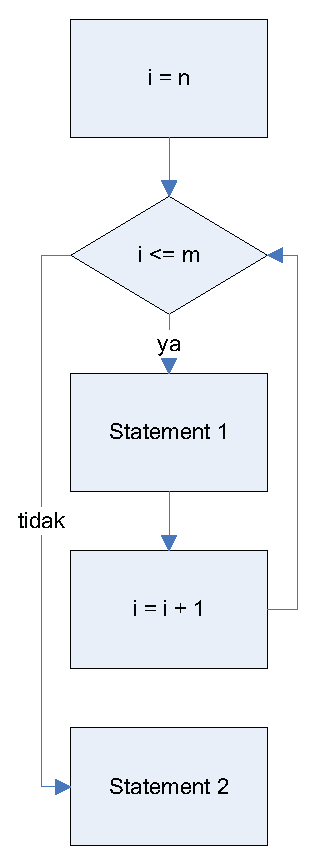
\includegraphics[scale=0.6]{fig/flowchart-FOR.eps}%
\caption{Flowchart For}%
\label{fig:flowchartFor}%
\end{figure}

\FloatBarrier
Untuk struktur \textit{while} bisa dilihat sebagai berikut.
\begin{tabbing}
\textbf{while} (Kondisi Logika)~~~~~~~~~~~~~~~\=\#Menjalankan perulangan selama kondisi benar\\
~~~~~statements\\
\textbf{end while}
\end{tabbing}

\FloatBarrier
\begin{contoh}
	\textbf{Penggunaan WHILE}
		\begin{algorithm}[H]
		\caption{PERULANGAN-WHILE-CETAK-1-SAMPAI-5()}
			\begin{algorithmic}[1]
			\STATE $i=1$
			\WHILE{$i<=5$}
				\STATE print $i$
				\STATE $i=i+1$
			\ENDWHILE
			\end{algorithmic}
		\end{algorithm}
\end{contoh}

Format bahasa Python untuk \textit{while} adalah sebagai berikut.

\begin{tabbing}
\textbf{while} (Kondisi Logika):~~~~~~~~~~~~~~~\=\#Menjalankan perulangan selama kondisi benar\\
~~~~~statements\\
\end{tabbing}

Contoh penggunaan \textit{while} dalam bahasa Python untuk mencetak menurun bilang 10 sampai 1 bisa dilihat di Listing \ref{lst:cetakBilanganTurun}.
\begin{listprog}{cetakBilanganTurun.py}
	\label{lst:cetakBilanganTurun}
	\begin{lstlisting}[language=Python]
		i = 10
		while(i>0):
			print i
			i = i - 1	\end
		#Hasil print berupa 10 9 8 7 6 5 4 3 2 1
	\end{lstlisting}
\end{listprog}


Untuk \textit{flowchart} \textit{while} bisa dilihat di Gambar \ref{fig:flowchartWhile}.
\begin{figure}%
\centering
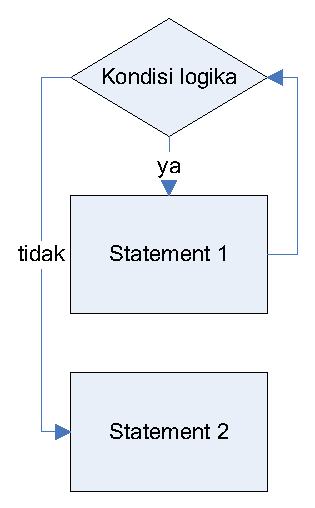
\includegraphics[scale=0.6]{fig/flowchart-WHILE.eps}%
\caption{Flowchart While}%
\label{fig:flowchartWhile}%
\end{figure}


\FloatBarrier
\subsection{Perulangan Bersarang}
Sebuah perulangan dapat memiliki perulangan di dalamnya dan perulangan yang di dalam tersebut juga dapat juga dapat memiliki perulangan lainnya di dalam. Perulangan yang di dalam tersebut tidaklah harus menggunakan pernyataan yang sama dengan perulangan induknya. Misalnya, boleh saja kita menggunakan pernyataan perulangan \textit{for} di dalam pernyataan perulangan \textit{while} dan juga sebaliknya. Algoritma berikut akan menunjukkan salah satu struktur perulangan bersarang.

\begin{tabbing}
\textbf{for} $i=n$ \textbf{to} $m$~~~~~~~~~~~~~~~\=\#Mengisi variabel i, dan lakukan perulangan sebanyak (m-n-1)\\
~~~~~\textbf{for} $j=n$ \textbf{to} $m$~~~~~~~~~~~~~~~\=\#Mengisi variabel j, dan lakukan perulangan sebanyak (m-n-1)\\
~~~~~statements\\
~~~~~\textbf{end for}\\
\textbf{end for}
\end{tabbing}

	
 
